% ==============================================================================
%  styles/cover.tex —— 封面版式
%  调用：\DisplayCover（开关在 main.tex，注释掉即可不显示封面）
%  要改的标题/作者/学生信息/课程/参考文献都在 main.tex 的“封面信息”区
% ==============================================================================

\newcommand{\LoneCoverSepI}{\resizebox{270pt}{4pt}{
\includegraphics{assets/pdf/separator_1.pdf}}}
\newcommand{\SSS}{\LoneCoverSepI}% 向后兼容别名
\newcommand{\LoneCoverSepII}{\resizebox{199pt}{!}{
\includegraphics{assets/pdf/cover_sep.pdf}}}
\newcommand{\FFF}{\LoneCoverSepII}% 向后兼容别名

% ---------------- 标题 ----------------
\newcommand{\TitleText}{%
	\fontsize{36}{12}\selectfont\color{qiancheng}\XeTeXinterchartokenstate=0
	\AvantGarde\addfontfeatures{LetterSpace=-5} \LoneTitleI{}
	\SSS \\[8pt]
	\SiYuan \LoneTitleII
}

% ---------------- 作者 ----------------
\newcommand{\AuthorText}{%
	\fontsize{15}{16}\selectfont\color{qiancheng}\XeTeXinterchartokenstate=0
	\AvantGarde\addfontfeatures{LetterSpace=-5} \LoneAuthor
}

% ---------------- 信息表（COURSE / NAME / STUDENT ID / DATE） ----------------
% 左列橙色标签（Avant Garde 加粗），右列内容（思源黑体加粗）用封面左侧三竖条最右那条的 hong 色。
\newlength{\InfoLabelW}   \setlength{\InfoLabelW}{96pt}
\newlength{\InfoValueW}   \setlength{\InfoValueW}{190pt}
\newlength{\InfoGap}      \setlength{\InfoGap}{14pt}

% \InfoRow{标签}{内容}
\newcommand{\InfoRow}[2]{%
	\makebox[\InfoLabelW][l]{%
		\fontsize{15}{15}\selectfont\bfseries
		\AvantGarde\XeTeXinterchartokenstate=0\color{qiancheng}#1}%
	\hspace{14pt}%
	\makebox[\InfoValueW][l]{%
		\fontsize{15}{15}\selectfont\bfseries
		\SiYuan\XeTeXinterchartokenstate=0\color{heise}#2}%
}

\newcommand{\InfoTable}{%
	\begin{tabular}[t]{@{}l@{}}
		\InfoRow{COURSE}{\LoneCourseI} \\[\InfoGap]
		\InfoRow{NAME}{\LoneStudentName} \\[\InfoGap]
		\InfoRow{STUDENT ID}{\LoneStudentID} \\[\InfoGap]
		\InfoRow{DATE}{\LoneDate} \\
	\end{tabular}%
}

% ---------------- 封面线 + 参考文献 + 致谢 ----------------
\newcommand{\ReferenceText}{%
	\FFF \\[14pt]
	\fontsize{9}{7}\selectfont\color{qiancheng}\AvantGarde\XeTeXinterchartokenstate=0 Reference: \\
	\fontsize{6}{7}\selectfont\color{heise}\AvantGarde\XeTeXinterchartokenstate=0 \LoneRefA \\
	\fontsize{6}{7}\selectfont\color{heise}\AvantGarde\XeTeXinterchartokenstate=0 \LoneRefB \\
	\fontsize{6}{7}\selectfont\color{heise}\AvantGarde\XeTeXinterchartokenstate=0 \LoneRefC \\[12pt]
	\fontsize{9}{7}\selectfont\color{qiancheng}\AvantGarde\XeTeXinterchartokenstate=0 Acknowledgements: \\
	\fontsize{6}{7}\selectfont\color{heise}\AvantGarde\XeTeXinterchartokenstate=0 \LoneAcknowledgements \\
}

% ---------------- 封面本体 ----------------
\newcommand{\makecover}{%
	\clearpage
	\thispagestyle{empty}
	\newgeometry{top=0pt, bottom=0pt, left=0pt, right=0pt}
	\defaultfontfeatures{LetterSpace=0, LetterSpaceLimit=-200}
	\begin{tikzpicture}[remember picture, overlay]
		\node[anchor=north west, inner sep=0pt, outer sep=0pt] at (current page.north west) {
			\resizebox{\paperwidth}{\paperheight}{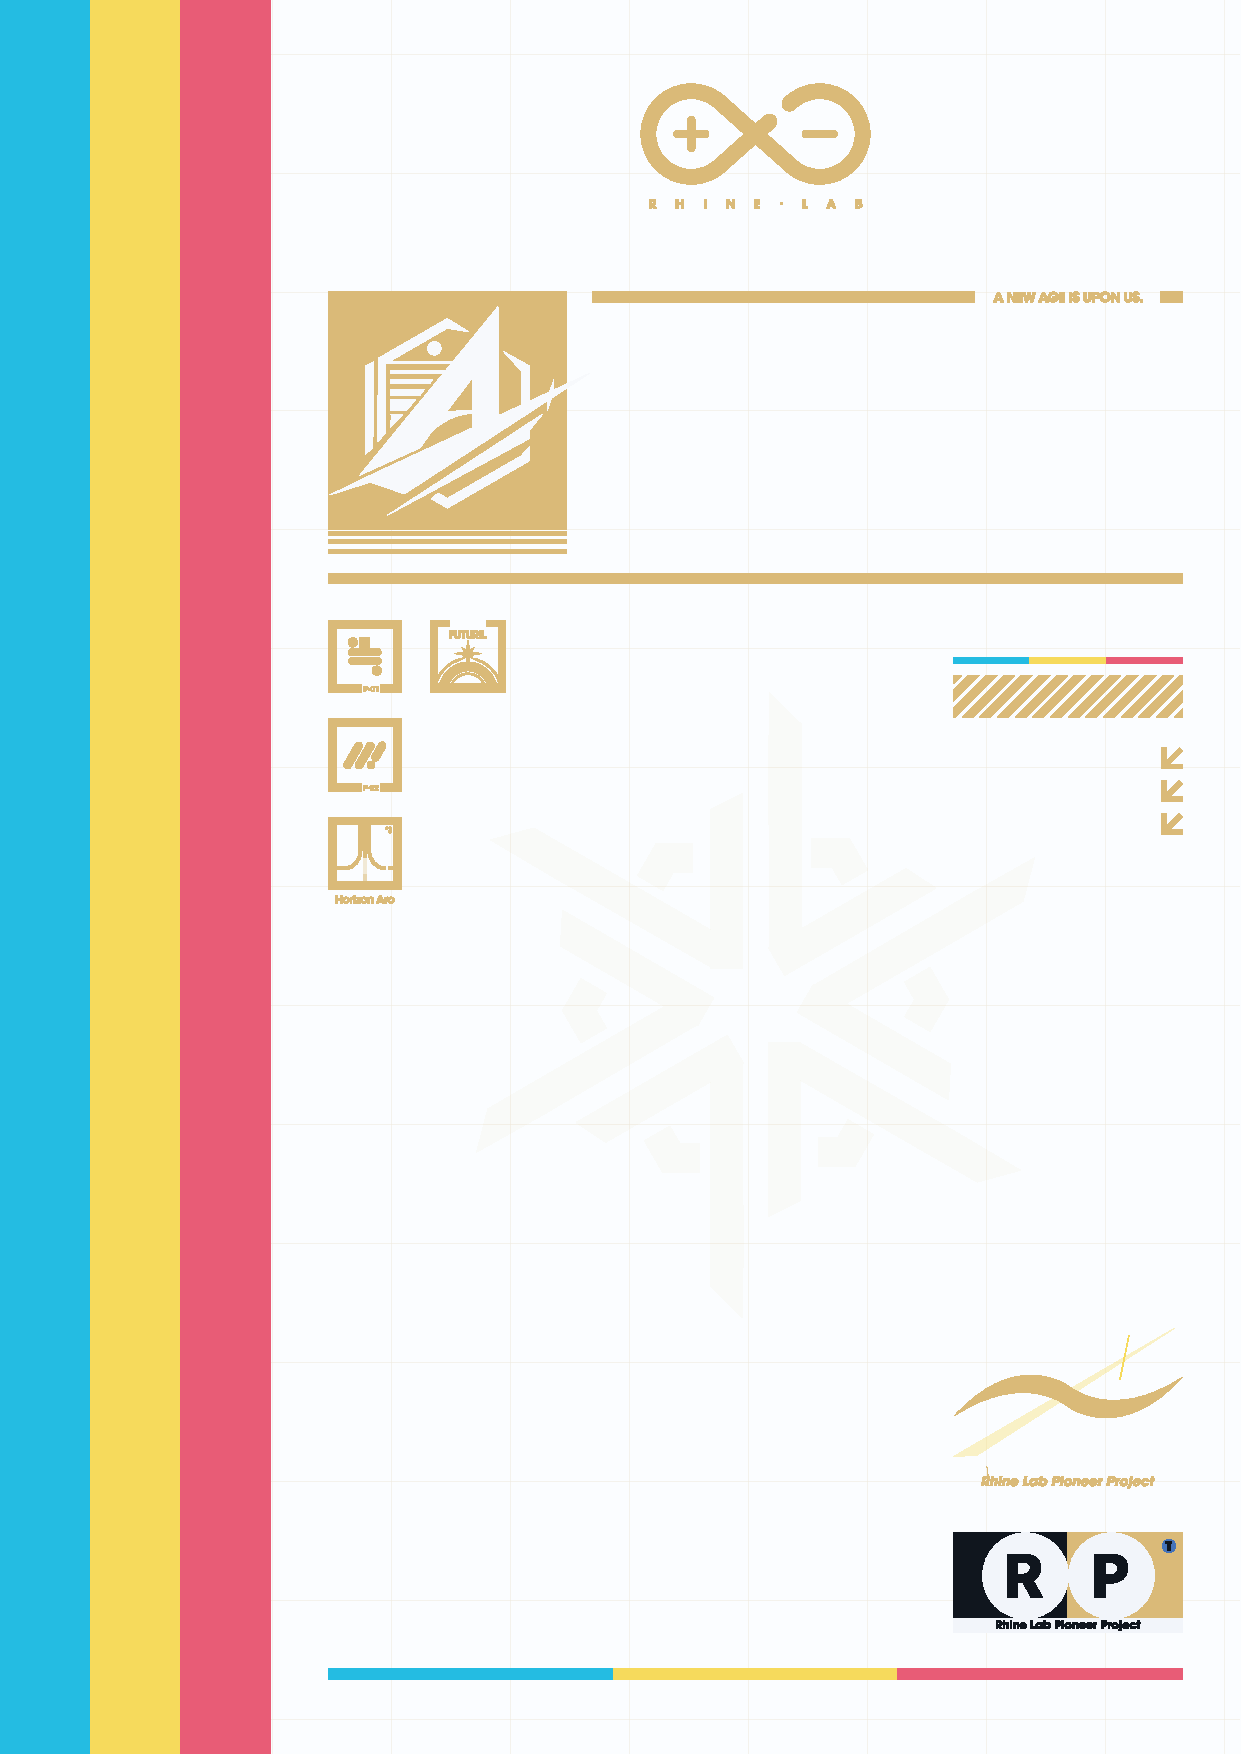
\includegraphics{assets/pdf/cover_bg.pdf}}
		};

		% ---- 标题 ----
		\node[
		anchor=north west,
		minimum width=280pt,
		minimum height=100pt,
		text width=280pt,
		inner sep=0pt,
		outer sep=0pt,
		align=left,
		] at ($(current page.north west) + (10.096cm,-5.4467cm)$) {\TitleText};

		% ---- 作者（标题右下） ----
		\node[
		anchor=north west,
		minimum width=110pt,
		minimum height=12pt,
		text width=110pt,
		inner sep=0pt,
		outer sep=0pt,
		align=center,
		] at ($(current page.north west) + (16.1444cm,-10.4991cm)$) {\AuthorText};

		% ---- 课程 / 姓名 / 学号 / 日期（页面中下方） ----
		\node[
		anchor=north west,
		inner sep=0pt,
		outer sep=0pt,
		align=left,
		] at ($(current page.north west) + (5.9cm,-18.6cm)$) {\InfoTable};

		% ---- 参考文献 / 致谢（左下角） ----
		\node[
		anchor=south west,
		minimum width=199pt,
		minimum height=11.8577pt,
		text width=199pt,
		inner sep=0pt,
		outer sep=0pt,
		align=left,
		] at ($(current page.north west) + (5.5611 cm,-27.6346cm)$) {\ReferenceText};
	\end{tikzpicture}

	\restoregeometry
	\clearpage
}

% ---------------- 显示开关 ----------------
% 在 main.tex 中注释掉 \DisplayCover / \DisplayTOC 即可隐藏对应页面
\newcommand{\DisplayCover}{\makecover}
\newcommand{\DisplayTOC}{%
	\clearpage
	\LoneInTOCtrue
	\newgeometry{left=2.1cm,right=0.95cm,top=5.8cm,bottom=2cm}%
	\makecustomtoc
	\clearpage
	\restoregeometry
	\LoneInTOCfalse
}
